\chapter{Introduction}
\blfootnote{Portions of this chapter appear as
J.H.\ Abel and F.J.\ Doyle III, ``A systems approach to analysis and control of mammalian circadian dynamics,'' \textit{Chemical Engineering Research and Design}, vol.~116, 2016. DOI:~10.1016/j.cherd.2016.09.033; and J.H.\ Abel, A.\ Chakrabarty, and F.J.\ Doyle~III ``Pharmaceutical-based entrainment of circadian phase via nonlinear model predictive control,'' submitted.
The text has been modified to provide a more thorough introduction.
% copyright info covered under personal use: https://www.elsevier.com/about/our-business/policies/copyright/personal-use
% double checked using get rights and content - all good
}

Circadian rhythms are endogenous oscillations in gene expression, metabolism, and behavior that allow an organism to adjust its internal state to predictable cyclic changes in the environment.
This advantageous feed-forward approach to life in a temporally cyclic environment allows an organism with a circadian rhythm to anticipate environmental variability and adjust its physiology without a time lag.
Circadian regulation of biological processes is therefore highly-conserved: these rhythms have been identified in diverse species from mammals, insects, plants, and fungi to prokaryotic cyanobacteria \cite{Reppert2002, Hardin2005, Harmer2000, Dunlap2004a}.
Although circadian clocks share common properties between species, the mechanistic origins and hierarchical complexity of these rhythms can vary significantly.
Prokaryotes have been shown to use minimal phosphorylation-based nontranscriptional oscillators, which may be reconstituted \textit{in vitro} \cite{Ishiura1998, Nakajima2005}.
Meanwhile, eukaryotic organisms employ transcriptional-translational feedback loops in addition to post-translational protein modification for timekeeping \cite{Dunlap1999, ONeill2011}.
In larger organisms such as mammals, circadian rhythms must be coordinated across cells and tissues, resulting in a complex yet robust circadian control system \cite{Welsh2010, Doyle2006}.
% end paragraph, talk about approaches

The inherently complex (i.e.\ involving nonlinearity and feedback) and stochastic (i.e.\ fundamentally involving randomness and noise) nature of these processes has necessitated mathematical approaches for understanding biological clocks, as their properties emerge from the often-imprecise interaction of numerous molecules and pathways.
Such approaches have included mechanistic and empirical process modeling \cite{Kronauer1999, Jewett1999, Leloup2003a, Gonze2003, Forger2005, To2007, Mirsky2009b,  Ko2010, Hirota2012a}, robustness and sensitivity analysis \cite{Leloup2003a, Gonze2006, Rougemont2007, Taylor2008a, Tidor2009, StJohn2013, Taylor2014a}, and optimal or feedback control \cite{Doyle2006, Bagheri2008, Bagheri2008a, Serkh2014, Zhang2016}.
%cite models, methods, tools, etc. essentially show that this is true here
This thesis presents recent advances in developing an understanding of, and artificially exerting control over, the mammalian circadian system through mathematical approaches.


\subsubsection*{On organization}
In this chapter, I begin by presenting a brief historical overview of the study of daily patterns of behavior, culminating with the identification of clock genes in multiple organisms in the 1990s.
I next define the general characteristics that constitute a circadian rhythm.
I then introduce biological generation of mammalian circadian rhythms, and also note how this structure compares to that of other organisms.
I present a mathematical framework for modeling and analysis of circadian dynamics based on the limit cycle oscillator, and present derivations for relevant quantities.
Finally, I discuss motivation for feedback control of circadian rhythms, and the components of a system to achieve this.

The ensuing dissertation is then divided into two main sections to reflect the two foci of my research.
In Section I, I present projects in fundamental biology toward the aim of understanding the structure and function of mammalian circadian rhythm generation and synchronization in the suprachiasmatic nucleus (SCN).
In Section II, I present a mathematical framework for taking control of this system, and derive results that aim to guide the development of this capability.
Future research aims are included separately for each Section.

My exact contributions are noted for each section so as to avoid claiming credit for the work of my dedicated and highly skilled collaborators.
The majority of this work has already been published, and for published chapters I have attempted to edit as little as possible for this volume.
This serves two purposes: consistency in the literature record and avoiding the introduction of new errors of my own making.

\subsubsection*{On notation}

Where possible, I have generally attempted to adopt a uniform notation throughout this thesis.
This has primarily affected the presentation of this Introduction: the notation has been changed from the original publication to match with Section II.
For the confused reader, I would recommend studying the original publications in detail: the notation in these is certainly internally consistent and self-contained.

\section{An introduction to circadian rhythms}

\subsection*{A brief history of circadian biology}
It has long been noticed that organisms adjust their physiology in accordance with day-night cycles.
Androsthenes of Thasos, an admiral in the navy of Alexander the Great, noted daily rhythms in leaf movements of \textit{Tamarindus indicus}, but did not suspect that these rhythms were more than a response to light \cite{McClung2006b}.
It was not until the 1700s that the first ``true'' chronobiological experiment was performed, demonstrating that rhythms in leaf movement are endogenous, rather than a response to the light-dark cycle \cite{de1729observation}.
In the following 200 years, endogenous rhythms in physiology were observed in more plant species, arthropods \cite{kiesel1894untersuchungen}, and eventually, rats \cite{richter1922behavioristic}.
By the mid 20th century, it was well-established that an unidentified endogenous process was driving the near-24 hour rhythms in behavior observed under constant conditions.

Perhaps the most important discovery in identifying the underlying basis of circadian rhythms was the discovery of the \textit{Period} (\textit{Per}) gene in \textit{Drosophila melanogaster} in 1971 \cite{Konopka1971}.
In a classic work, Konopka and Benzer demonstrated that inducing mutations in a single gene on the \textit{Drosophila} X chromosome can induce lengthened, shortened, or abolished circadian eclosion rhythms in constant darkness.
Furthermore, these mutations conferred altered circadian period phenotypes in adults, indicating that an underlying genetic oscillator drives circadian rhythms, and that this oscillator persists through metamorphosis.
It was this and the ensuing studies that led to the discovery of the autoregulatory function of \textit{Per} \cite{Hardin1990}, the discovery of the gene involved in its nuclear localization (\textit{Timeless}) \cite{Vosshall1994}, and the 2017 Nobel Prize in Physiology or Medicine.
In this same timeframe, the genetic basis of the mammalian clock was identified as a transcription-translation feedback loop analogous to the \textit{Per}/\textit{Timeless} feedback loop of \textit{Drosophila}.
A homologous \textit{Per} gene was identified in mammals, and \textit{Cryptochrome} was identified as its co-regulator \cite{Vitaterna1999}.
Furthermore, homologs of the \textit{Clock} gene were identified as the transcriptional activator in both mammals and \textit{Drosophila} \cite{Vitaterna1994, Darlington1998}.

Since the identification of the key transcriptional pathways of the mammalian circadian clock, much effort has focused on elucidating the complex genetic architecture surrounding the clock \cite{Zhang2009, Takahashi2016}.
The circadian oscillator has been found to widely regulate transcription within mammals, and approximately 10\% of all transcripts cycle with circadian periodicity \cite{Lowrey2004}.
This is perhaps unsurprising, as genetic evidence suggests that circadian rhythms evolved in concert with peroxiredoxin oxidation-reduction cycles \cite{Edgar2012}.
Because cycles in metabolic regulation may have enabled archaic organisms to survive oxidative stress cycles in a newly-aerobic environment, circadian rhythms are deeply integrated within cellular and organismal metabolic networks.

\subsection*{Properties of the circadian clock}
Circadian rhythms are distinguished from other periodic biological processes by several criteria \cite{Dunlap2004}.
First, circadian rhythms are endogenous, that is, they are self-sustained even in constant environmental conditions.
Second, circadian clocks are entrainable and shift in phase or period to align with environmental cycles through cues referred to as \textit{zeitgebers}\footnote{Trans. German: Time-givers}.
Third, they are traditionally considered to be temperature-compensated, meaning oscillator period is insensitive to changes in temperature in the external environment.
This property has recently drawn renewed scrutiny in the past 15 years following evidence that temperature cycles can entrain cell-autonomous circadian oscillators \cite{Herzog2003}.
Finally, circadian rhythms have oscillatory periods of approximately, though often not exactly, 24 hours.
Counterintuitively, a near-24h period may be more advantageous than an exactly-24h period, as it provides increased stability of entrained phase angle \cite{Dunlap2004}.

\section{The mammalian circadian control system}

In mammals, circadian rhythms are generated within individual cells by a network of interlocked genetic feedback loops \cite{Dunlap1999, Ko2006, Mohawk2012}.
These cell-autonomous clocks are responsible for regulation of genetic expression and metabolic processes in local tissue.
For example, circadian regulation of glucose metabolism is localized to liver tissue, and the deletion of core clock genes in only liver tissue is sufficient to abolish circadian rhythms in expression of glucose regulatory genes \cite{Lamia2008a}.
This view is supported by studies demonstrating that rhythmic gene expression profiles are tissue-specific \cite{Panda2002, Ueda2002}.
Cellular rhythms are coordinated across tissues in the body and entrained to environmental rhythms through signals from the brain.
The hypothalamic suprachiasmatic nucleus (SCN) is considered the ``master clock'' in mammals: it is responsible for entraining to light inputs and maintaining synchrony among the cell-autonomous oscillators in peripheral tissues throughout the body \cite{Welsh2010}.
Peripheral tissues receive local inputs in addition to SCN signals, for example, cells in the liver may be entrained by rhythmic feeding independently of the SCN \cite{Stokkan2001}.
Finally, it is thought that peripheral clocks exert a degree of feedback into the SCN, though whether this is direct or indirect remains unknown \cite{Green2008}.

\subsection*{A need for understanding and control of the clock}
It is estimated that approximately 10\% of all mammalian transcripts are under circadian regulation \cite{Lowrey2004}.
With such widespread influence, it is unsurprising that circadian rhythms play an important role in human health and disease.
In particular, high amplitudes of circadian transcription factors in peripheral tissues are desirable for good metabolic health.
Mice lacking circadian rhythms due to core clock gene knockouts, or with diminished circadian amplitude due to diet or age have been shown to develop diseases, including metabolic syndrome and diabetes \cite{Marcheva2010, Hatori2012, Chang2013}.
Similarly, lifestyle factors such as shift work can cause misaligned circadian cues, resulting in diminished amplitude of circadian oscillation, and ultimately, adverse health outcomes \cite{Green2008, Pan2011, Mukherji2015}.
Neurological diseases such as posttraumatic stress disorder (PTSD), depression, and addiction are also associated with circadian disregulation  \cite{Wulff2010,Yehuda1996, Rosenwasser2010}.
Thus, a general aim of the study of the circadian clock is the development of pharmacological or behavioral therapies for maintaining high-amplitude circadian rhythms, or easing the effects of circadian phase resetting during jet-lag or shift work.
Relatedly, there is interest in how circadian rhythms affect drug metabolism and efficacy, especially with respect to cancer medication due to circadian control of cell cycles \cite{Lemmer1991, Levi2010}.
To develop such therapies, the mammalian circadian clock must be investigated mechanistically as a dynamical system.



Circadian rhythms in mammals are generated within individual cells by interlocked transcriptional-translational feedback loops \cite{Ko2006}.
The cell-autonomous genetic clock is largely conserved across cell types, with the notable exception of red blood cells, which lack a nucleus and may compensate with a non-transcriptional clock \cite{Neill2011}.
Although the core clock is conserved, the genes under clock control may vary with cell type, creating a temporal architecture of gene expression across the body.

\subsection*{The cell-autonomous circadian clock}

\begin{figure}[p] 
    \begin{center}
        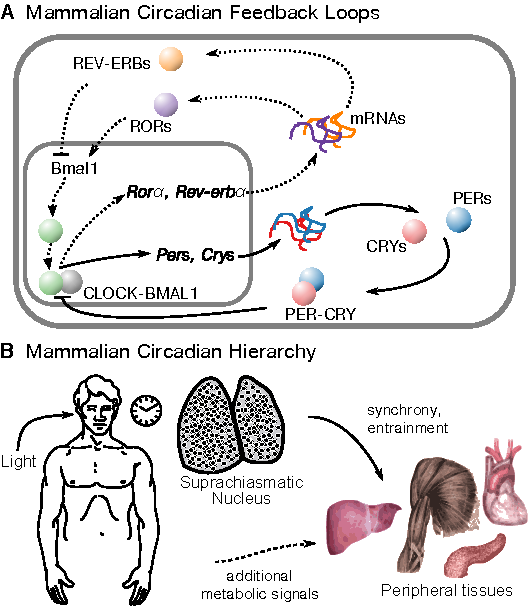
\includegraphics[width=90mm]{chap1/figures/figure_1_clock_hierarchy.pdf}
    \end{center}
    \caption{Schematic of the mammalian cell-autonomous clock and circadian system hierarchy.
        (\textbf{A}) Two interlocked feedback loops comprise the mammalian circadian oscillator: the PER-CRY negative feedback loop (solid lines), and the CLOCK-BMAL1 positive feedback loop (dotted lines). Diagram adapted from \cite{Ko2006}. 
        (\textbf{B}) The suprachiasmatic nucleus of the brain is the mammalian ``master clock,'' responsible for entrainment to external light cycles and synchronizing peripheral oscillators such as those within the liver, muscle, heart, and pancreas.
        Within the SCN, neurons exchange neuropeptidergic and electrical signals to maintain synchrony.
   \label{fig:hierarchy} }
\end{figure}

A schematic of the core clock is shown in Figure \ref{fig:hierarchy}A.
The interlocked positive (dotted lines) and negative transcriptional feedback loops (solid lines) are considered the primary source of circadian oscillation \cite{Mohawk2012, Ko2006}.
Within the negative loop, isoforms of the \textit{Period} (\textit{Per1,2,3}) and \textit{Cryptochrome} (\textit{Cry1,2}) are transcribed and translated, and form heterodimers.
PER-CRY heterodimers re-enter the nucleus, and repress transcription of Enhancer box (E box) genes including \textit{Per} and \textit{Cry} through sequestration of E box activator CLOCK-BMAL1 by dissociated CRY \cite{Ye2011}.
Over time, nuclear PER and CRY is degraded, allowing transcription to resume.
This negative loop is balanced by an interlocked positive feedback loop regulating the expression of \textit{Bmal1}.
In this loop, E box-controlled genes \textit{Rev-erb}$\alpha$ and \textit{Ror}$\alpha$ repress and promote \textit{Bmal1} transcription, respectively, through competitive binding to the ROR/REV-ERB Response Element (RRE) in the \textit{Bmal1} promoter \cite{Emery2004}.
Collectively, the genes \textit{Per}, \textit{Cry}, \textit{Clock}, and \textit{Bmal1} are considered the core circadian clock.

It is important to note here that new evidence is emerging which downplays the primacy of transcriptional activity in circadian oscillation \cite{Dunlap2017}.
Recent studies have shown that limited oscillation may still occur in the absense of transcriptional oscillations of core clock genes, likely due to feedback loops involving phosphorylation of the products of core clock genes \cite{Fan2007, Ode2017, Ode2017a}.
While this may yet become a monumental shift in our understanding of the clock, it is important to also note that the behavior of the clock, whether transcriptional or phosphorylational, exhibits the mathematical properties of a limit cycle oscillator, and so the approaches described herein may be applied analogously to such a phosphorylational system, should it be identified as the efficient cause of circadian oscillation.

The core clock regulates cellular transcription of clock-controlled genes (CCGs) via RREs, E boxes, and D boxes (DBP binding elements) \cite{Ueda2005}. 
Because the transcription factors corresponding to these elements peak at different circadian times, transcription of genes may be partitioned into various times of day.
The core clock is also affected by a wide variety of cell type-specific transcription factors or posttranslational regulators. 
A genome-wide RNAi screen identified hundreds of genes with phenotypic effects on clock period or amplitude, indicating that clock pathways are highly interconnected with other, often tissue-specific metabolic pathways \cite{Zhang2009}.


\begin{table}[t]
    \small
    % table is here so that latex puts it on the right page
    \caption{A non-exhaustive list of notable mammalian circadian models demonstrating the range in scale and scope of such models. While not specific to circadian oscillation, the structure of the Goodwin oscillator is a common framework for circadian analysis.}
    \begin{tabular}{l c c l} 
         & Dynamic & Kinetic &  \\
         Reference & States & Parameters & Model Form \\
        \hline
        Goodwin 1965 \cite{Goodwin1965} & 3 & 6 & general limit cycle ODE model\\
        Kronauer \textit{et al.} 1999 \cite{Kronauer1999} & 3 & 9 & ODE limit cycle with light response \\
        Leloup and Goldbeter 2003 \cite{Leloup2003a} & 16 & 53 & mammalian mechanistic ODE model\\
        Forger and Peskin 2005 \cite{Forger2005} & 73 & 36 & mammalian mechanistic CME model\\
        To \textit{et al.} 2007 \cite{To2007} & 17/cell & 62 & multicellular mammalian ODE model\\
    \end{tabular} 
\end{table}


\subsection*{Stochasticity in the clock}
Macroscale chemical processes may be approximated with continuous chemical kinetics, however, 
the low copy number of genes, transcripts, and proteins within an individual cell results in considerable
deviation from continuous kinetics \cite{Elowitz2002}.
Stochasticity, or molecular noise, caused by the discrete nature of biochemical 
reactions, is referred to as \textit{intrinsic} stochasticity.
Although circadian rhythms are precise at the organism-scale, there is a significant 
degree of intrinsic stochasticity in circadian oscillation at the single-cell scale.
The cycle-to-cycle variation in circadian period within a single cell is due to intrinsic stochasticity \cite{Herzog2004}.
Intrinsic stochasticity may be captured computationally through the use of stochastic simulation algorithms \cite{Forger2005, Gonze2006}.
Cellular reactions are also subject to \textit{extrinsic} stochasticity, caused by differences
between cells or within the microscopic environment, including gradients in temperature, 
or differences in cell cycle phase, cell size, or organelle distribution.
Extrinsic stochasticity may be simulated by introducing a variability in model parametrization.
Intrinsic and extrinsic variability have been studied in the circadian clock experimentally 
\cite{Herzog2004, Welsh2004} and computationally \cite{Barkai2000, Forger2005, Gonze2006, Rougemont2007, Ko2010, Abel2015a, StJohn2015}.
Within the circadian system, communication between cells and tissues allows the maintenance 
of a precise circadian phase, and adaptation to environmental cues.


\subsection*{Hierarchy of clocks in the body}
Mammalian circadian hierarchy, shown in Figure~\ref{fig:hierarchy}B, enables the coordination of circadian oscillation through the organism.
The suprachiasmatic nucleus (SCN), the ``master clock,'' consists of approximately 20,000 neurons within the hypothalamus.
Neurons within the SCN synchronize spontaneously and therefore maintain tissue-scale oscillation indefinitely \textit{in vitro}, whereas other tissues which lack intercellular communication display a damped oscillation likely due to gradual dephasing \cite{Welsh2004, Yoo2004}. 
SCN neurons exchange neuropeptidergic, neurotransmitter, and electrical signals to synchronize \cite{Welsh2010}.
Molecular signals of primary importance are vasoactive intestinal peptide (VIP) and $\gamma$-aminobutyric acid (GABA) \cite{Aton2005, Aton2006, Evans2013, Myung2015}.
The SCN is commonly divided into two regions: a ventral ``core'' and a dorsal ``shell,'' which differ in neuropeptide expression and response, and neuronal network structure \cite{Albus2005, Welsh2010, Myung2015, DeWoskin2015, Evans2013, Abel2016}.
The SCN entrains through its core region receiving light input from the retinohypothalamic tract (RHT) \cite{Welsh2010}.
The SCN then adjusts its phase of oscillation to match light cues, and the shell region outputs time of day cues to connected brain regions and ultimately the rest of the body \cite{Evans2015}.

Peripheral tissues sustain oscillation in the absence of a functional SCN, however, signals from the SCN are necessary to maintain a coherent phase \cite{Welsh2010}.
These signals from the SCN include sympathetic and parasympathetic pathways, hormonal rhythms, and temperature \cite{Mohawk2012}.
In addition to signals from the SCN, peripheral tissues receive local metabolic cues which help to establish circadian phase.
Glucose, glucocorticoids, insulin, and other common metabolic factors have been shown to influence the clock, and it is possible that multiple metabolic signals are simultaneously responsible for modulating peripheral clocks \cite{Green2008, Bass2010}.
Restricted feeding in rodents has been shown to effectively decouple liver cells from the SCN and shift circadian phase by nearly 180$^\circ$, indicating that metabolic cues form an important component of the circadian system \cite{Damiola2000}.

\section{Quantitative analysis of circadian dynamics}

In the past several decades, significant advances in understanding circadian rhythms have been made through the use of mathematical modeling.
Here, we present an introduction to sensitivity analysis and modeling of the circadian clock, with a focus on ordinary differential equation models.
Section \ref{sec:31} introduces the concept of a limit cycle oscillator, a dynamical system commonly used to describe circadian clockwork.
Section \ref{sec:32} introduces a variety of quantitative tools for the analysis of a single limit cycle oscillator, and \ref{sec:33} expands upon these tools for the analysis of a population of oscillators.
Sections \ref{sec:34} and \ref{sec:35} provide derivations of the tools introduced in \ref{sec:32} and \ref{sec:33}, respectively, and comment on how these quantities may be calculated.
For the casual reader, \ref{sec:34} and \ref{sec:35} may be omitted without loss of qualitative understanding.


Circadian clock dynamics are commonly modeled through coupled nonlinear equations.
Broadly, clock models may be empirical (i.e., designed to capture clock behavior without regard for the underlying physical system), or mechanistic (i.e., comprised of the underlying species and their mathematical relationships).
Furthermore, these models may consist of deterministic ordinary differential equations (ODEs) \cite{Kronauer1999, Jewett1999, Leloup2003a, To2007, Mirsky2009b, Kim2012, Hirota2012a}, a discrete stochastic chemical master equation (CME) \cite{Forger2005, Gonze2006, Ko2010, Abel2015a}, or Langevin stochastic differential equations (SDEs) \cite{Westermark2009, Koeppl2011}.
Stochastic approaches are generally utilized in cases where intrinsic molecular noise is thought to be significant.
A description and the dimensions of five notable circadian models are provided in Table 1.

Irrespective of these possibilities, the circadian clock is primarily modeled as a deterministic set of ODEs comprising a limit cycle oscillator.
This is because the circadian oscillator exhibits limit cycle-like behavior: it has a self-sustained oscillation with stable waveform and amplitude, the oscillator manifold is attractive, and perturbations to oscillation result in a phase shift.
The dynamics of a limit cycle oscillator are additionally useful for explaining entrainment and phase and amplitude response behavior of the circadian oscillator.


\subsection*{The limit cycle oscillator\label{sec:31}}

Limit cycle oscillators are not unique to biology, for example, they have been utilized to describe oscillatory chemical reactions \cite{Field1974}, electrical circuits \cite{VanderPol1926}, and earthquakes \cite{Huang1990}.
As such, some of the following tools were first conceptualized outside of the context of biological rhythms.
For this work, we are exclusively interested in tools developed to describe attractive limit cycles.
An attractive limit cycle oscillator consists of a set of coupled ODEs of the form:
\begin{equation}
    \label{eq:odes}
    \frac{dx}{dt} = f(x, t, p),
\end{equation}
which satisfies:
\begin{equation}
    \label{eq:lc}
    \lim_{t\to\infty}[x(t) - x(t-T)]=0.
\end{equation}
The steady state limit cycle is therefore the closed oscillatory path $\Gamma\subset\mathbb{R}^n$ which is traversed with a period of $T$, where $T$ is the smallest positive value for which \eqref{eq:lc} holds.
For mechanistic models, $x \in \mathbb{R}^n$ is a vector of state concentrations, $p \in \mathbb{R}^m$ are kinetic parameters, and $\dot x = f(x,p)$ are differential material balance equations, of the form:
\begin{equation}
    \label{eq:kin}
    \frac{dx_i}{dt} = r_{x,in}-r_{x,out} +r_{x,generation}-r_{x,consumption}
\end{equation}
for each of $n$ species. 
The rate terms comprising the right hand side of \eqref{eq:kin} may follow mass-action, Michaelis-Menten, or Hill kinetics, providing an explicit mathematical analogy with the treatment of a continuous stirred tank reactor (CSTR) system.
Here, the concentrations of mRNA and protein species correspond with the reactants and products in a CSTR, and the volume of the subcellular compartment in which each species resides corresponds to CSTR volume.
However, concentrations are often provided in arbitrary concentration units for simplicity without loss of information.
Empirical models need not conform to this physicality, and as such the Van der Pol oscillator is commonly used \cite{Kronauer1999}.
For simplicity, we will continue with our treatment of a mechanistic model, though the same tools apply to empirical models differing only in interpretation.


Each unique point $x_0$ on the stable limit cycle $\Gamma$ corresponds to a unique phase $\phi_0 \in\mathbb{S_1}=[0,2\pi)$, with the corresponding mapping $\Phi : \Gamma \to \mathbb{S}^1$.
Let $\gamma(t,x_0)$ denote the solution of system \eqref{eq:odes} with initial condition $x(0)=x_0\in\Gamma$.
Then, a time-dependent phase variable may be established
\begin{equation}
\phi(t) = \Phi[\gamma(t,x_0)].
\end{equation}
Intuitively, phase increases linearly with respect to time along the path $\Gamma$: 
\begin{equation}
    \frac{d\phi}{dt} = \omega,
\end{equation}
where $\omega = 2\pi/T$ is the radial frequency.
This yields particular solutions of the form
\begin{equation}
    \phi(t) = \omega t +\phi_0 \qquad \mod 2\pi
\end{equation}
where $\phi_0 = \Phi(x_0)$. 
Finally, let $x^0 \in\Gamma$ denote the arbitrary point on the limit cycle for which $\Phi(x^0) = 0$.\footnote{On notation: it is important to remember that $x_0$ is an arbitrary point on $\Gamma$, and $x^0$ is the particular point on $\Gamma$ for which $\phi=0$. Thus, trajectory $\gamma(t,x_0)$ is any arbitrary trajectory along $\Gamma$, but $\gamma(t,x^0)$ is the trajectory along $\Gamma$ for which $\phi(0)=0$.}

\subsection*{Sensitivity analysis of limit cycle models \label{sec:32}}

For oscillatory systems, most dynamic biological data are concerned with how the period of oscillation is affected by a permanent change in parameter values \cite{Zhang2009, Hirota2012a}, or how the phase or amplitude of oscillation is affected by temporary changes in state variable concentrations or parameter values \cite{Pittendrigh1976, Jewett1999, Vitaterna2006, Comas2006}.
Sensitivity analysis of dynamical systems is traditionally concerned with how a solution to differential or differential-algebraic equations varies with respect to perturbations in initial state or parameter values, and these biological quantities may be described within a sensitivity analysis framework.


Biologically relevant oscillatory sensitivity metrics include: phase change in response to a state perturbation (for example, the one-time addition of a clock protein) $\frac{d\phi}{dx}$; phase change in response to a temporary parameter perturbation (for example, applying a light pulse to photosensitive cells) $\frac{d}{dt}\frac{d\phi}{dp}$; amplitude change in response to a state perturbation $\frac{dA}{dx}$; amplitude change in response to a temporary parameter perturbation $\frac{d}{dt}\frac{dA}{dp}$; period change in response to a permanent parameter change (for example, knockout of a clock protein isoform) $\frac{dT}{dp}$.
The phase shift $\Delta\phi$ for a temporary change in parameter value converges asymptotically in time.
However, because period $T$ and orbit $\Gamma$ are dependent on parameterization, a permanent change in parameter value will result in the phase change $\Delta\phi$ accumulating \cite{Taylor2008a, Tidor2009}.
The phase response of a system to state or parameter perturbations occurring at different phases is commonly called a phase response curve (PRC), and its amplitude equivalent may be called an amplitude response cure (ARC).

By combining these sensitivity metrics with biological investigations, mathematical models may be used to guide experimentation, predict system behavior under new conditions, identify the roles of novel genes within the biological circuit, or uncover the mechanisms of drug action.
In Section II, we additionally show how the infinitesimal parametric phase response curve $\frac{d}{dt}\frac{d\phi}{dp}$ may be used to exert control over the circadian system.
Sensitivity analysis may be further expanded to describe changes in probabilistic behavior of discrete stochastic systems described by the chemical master equation \cite{Gunawan2005}.
These metrics are necessarily unique for stochastic systems, as higher moments of the proability distributions of each state may vary while the first moment does not.





\subsection*{Analysis of cellular populations\label{sec:33}}
Thus far, we have treated the circadian clock as a single deterministic limit cycle oscillator.
This limit cycle oscillator may be interpreted as representing the population-scale circadian oscillation, or alternately the oscillation within a single cell.
Physically, each cell contains a noisy oscillator, which exhibits both intrinsic and extrinsic stochasticity.
In some cases, simultaneously examining population-scale and single-cell dynamics through mathematical analysis of a population of limit cycle oscillators allows further insight into clock function or control.

In the SCN, coherent population-scale oscillation is self-sustained, due to intercellular communication driving synchrony \cite{Welsh2010}.
In peripheral tissues, however, the lack of paracrine signalling results in a gradual damping of population-scale oscillation, as the cells comprising the population require external signals to maintain a synchronized phase \cite{StJohn2015}.
Cultured circadian reporter cells similarly lack intercellular signalling, thus these cultures must be examined through the dual lens of population and single-cell effects.
For example, a temporary perturbation to cultured reporter cells such as a light pulse will have two effects on the amplitude of bioluminescence: a cellular-scale effect due to the deviation from the limit cycle, and a population-scale effect due to the condensing or dispersing of cellular phases \cite{Pulivarthy2007,Ukai2007,StJohn2014b}.
The single-cell effect will be transient, due to relaxation to the limit cycle, but the population synchrony effect will persist well after the pulse has ended.

These effects may be quantified through the use of previously-discussed sensitivity metrics.
For example, a perturbation to cells within a region of negative slope of the single-cell PRC will result in increased population synchrony and thus increased population amplitude, whereas a positive slope will decrease population synchrony.
Thus, the slope of the single-cell PRC dictates the angle of entrainment for a population of oscillators.
Computational methods have been developed to distinguish between single-cell and population-scale effects on amplitude and phase \cite{StJohn2014b}, and a derivation of these methods is provided in Section \ref{sec:35}.



\subsection*{Mathematical treatment and sensitivity analysis for limit cycle models\label{sec:34}}

In this section, we provide derivations for the calculation of period, phase, and amplitude sensitivity, as introduced in \ref{sec:32}.
We begin by defining a local, first-order sensitivity matrix $\mathbf{S}$ as:
\begin{equation}
    s_{i,j}(t,\alpha) = \frac{\partial x_i(t,\alpha)}{\partial \alpha_j} = \lim_{\epsilon\to 0}\frac{x_i(t, \alpha+\epsilon e_j) -x_i(t, \alpha)}{\epsilon}
\end{equation}
where $\alpha$ may be any linear combination of model parameters and/or initial conditions, and $e_j$ is the $j$th unit vector \cite{Tidor2009,Taylor2008a}.
The sensitivity matrix with respect to state initial conditions, $\mathbf{S_x}\in\mathbb{R}^{n\times n}$, may be computed directly, by integrating
\begin{equation}
    \label{eq:sx}
    \frac{d\mathbf{S_x}(t)}{dt} = \mathbf{J}(x)\mathbf{S_x}(t) + \frac{\partial f(x,p)}{\partial x(0)},
\end{equation}
where $\mathbf{J}\in\mathbb{R}^{n\times n}$ is the Jacobian matrix with element $J_{k,i} = \frac{\partial f_k(x(t),p)}{\partial x_i}$ and with initial condition $\mathbf{S_x}(0)=\mathbf{I}$, the $n\times n$ identity matrix \cite{Rabitz1983}.
The parametric sensitivity matrix (denoted $\mathbf{S_p}\in\mathbb{R}^{n\times m}$) may be solved similarly, by integrating
\begin{equation}
    \label{eq:sp}
    \frac{d\mathbf{S_p}(t)}{dt} = \mathbf{J}(x)\mathbf{S_p}(t) + \frac{\partial f(x,p)}{\partial p},
\end{equation}
with zero initial condition \cite{Rabitz1983, Tidor2009}.
In some cases, the direct solution of $\mathbf{S}$ may not be practical, and an alternate formulation using a Green's function approach yields advantages \cite{Rabitz1983}.


%
The parametric period sensitivity $\frac{dT}{dp}$ may be calculated by solving the boundary value problem:
\begin{equation}
%
    \begin{bmatrix}
        \mathbf{M} - \mathbf{I} & f(x^0, p) \\[6pt]
        \frac{\partial f_i(x^0, p)}{\partial x} & 0 
    \end{bmatrix}
    \begin{bmatrix}
        \mathbf{S_{p,0}} \\[6pt]
        \frac{dT}{dp}
    \end{bmatrix}
        =
    \begin{bmatrix}
        -\mathbf{S_{p}}(T) \\[6pt]
        -\frac{\partial f_i(x^0, p)}{\partial p}
    \end{bmatrix}
%
\end{equation}
where $x^0\in\Gamma$ is the initial condition on the limit cycle as previously defined.
Here, $\mathbf{M}$ is the monodromy matrix of the sensitivity system parameterized by $p$, $\mathbf{I}$ is the $n\times n$ identity matrix, and $\mathbf{S_p}(T)$ is the solution to \eqref{eq:sp} integrated to time $T$ from initial condition $\mathbf{0}$.
Solving this system yields the desired period sensitivities as well as the initial conditions for parametric sensitivities $\mathbf{S_{p,0}}$.
For a detailed derivation of this result, I refer the reader to Ref.~\cite{Tidor2009}.

\subsubsection*{Phase response to state and parameter perturbations}
Because a limit cycle oscillator is attractive, perturbations away from the limit cycle will eventually return to the closed path $\Gamma$.
Thus, the concept of phase may be extended to any point within the region of attraction (excluding the stationary point for which $\frac{dx}{dt}=\mathbf{0}$).
Let trajectory $\theta(t,x_a)$ be the time evolution of point $x_a\notin\Gamma$, with dynamics given by \eqref{eq:odes}.
The asymptotic phase of point $x_a$, denoted $\phi_a$, is equal to the initial phase of the trajectory $\gamma(t, x_0)$ to which the trajectory $\theta(t,x_a)$ ultimately converges.
This yields the asymptotic phase mapping $\mathit{\Phi}(x_a)\in[0,2\pi)$.
That is, 
\begin{equation}
    \phi_a = \mathit{\Phi}(x_a) = \Phi(x_0),
\end{equation}
subject to
\begin{equation}
    0 = \lim_{t\to\infty}||\theta(t, x_a) - \gamma(t, x_0)||.
\end{equation}

A phase response curve (PRC) may therefore be calculated by a method of small perturbations: applying an identical perturbation in species concentration or parameter at each phase, and calculating the resulting phase shift $\Delta\phi$.
The infinitesimal PRC, the response to infinitesimal perturbations in species concentration or parameter value, is defined in \cite{Taylor2008a} for species $i$:
\begin{equation}
    \frac{d\phi}{dx_i} = \lim_{\Delta x_i\to 0} \frac{\Delta\phi}{\Delta x_i},
\end{equation}
or for parameter $j$:
\begin{equation}
    \frac{d}{dt}\frac{d\phi}{dp_j} = \lim_{t_p,\Delta p_j\to 0} \frac{\Delta\phi}{t_p \Delta p_j},
\end{equation}
where $t_p$ is the duration of the parameter perturbation.
Usefully, these quantities are related \cite{Taylor2008a}:
\begin{equation}\label{eq:prccomp}
    \frac{d}{dt}\frac{d\phi}{dp_j} = 
    \frac{d}{dt}\frac{d\phi}{dx}\frac{dx}{dp_j} =
    \frac{d\phi}{dx}\frac{df}{dp_j},
\end{equation}
necessitating only the calculation of the state impulse PRC.
This may be done through solving \eqref{eq:sx} using its Green's function formulation \cite{Rabitz1983}.
The homogeneous problem\footnote{On notation:
    I have chosen to use $t$ and $t'$ consistently with \cite{Rabitz1983,Kramer1984}, but note that our $t$ is the equivalent of $T$, and our $t'$ is the equivalent of $t$ in \cite{Taylor2008a}. $T$ here, as in \cite{Rabitz1983,Kramer1984}, refers to the period of oscillation.
            } 
is
\begin{equation}\label{eq:green}
    \frac{d}{dt}\mathbf{K}(t,t') = \mathbf{J}(\gamma(t,x^0))\mathbf{K}(t,t'),
\end{equation}
with $t>t'$ and initial condition $\mathbf{K}(t',t') = \mathbf{I}$, which admits the $n$ linearly-independent solutions to \eqref{eq:sx} as the columns of the kernel $\mathbf{K}$.
Since $t'\leq t$, an adjoint strategy is simpler than solving the integral form of \eqref{eq:green} \cite{Kramer1984}:
\begin{equation}
    \frac{d}{dt'}\mathbf{K}^\ast (t',t) = -\mathbf{K}^\ast (t',t)J(\gamma(t',x^0)), \quad \mathbf{K}^\ast (t,t) = I, \quad t' \leq t.
\end{equation}
This system may integrated backwards from $t'=t$ to $t'=0$ to solve for the adjoint matrix $\mathbf{K}^\ast$.
The infinitesimal PRC is then found from:
\begin{equation}\label{eq:siprc}
    \frac{d\phi}{dx_i} = \lim_{t\to\infty} \frac{K_{ki}^\ast (t',t)}{f(\gamma_k(t,x^0))},
\end{equation}
and thus we need only solve for one row of $\mathbf{K}^\ast$ \cite{Taylor2008a,Kramer1984}.
In the limit $t\to\infty$, \eqref{eq:siprc} is $T$-periodic as it reaches the limit cycle.
In practice, the adjoint solution approaches its limit cycle rapidly and this can be approximated by integration for three periods \cite{Taylor2008a}.
We note that as in \cite{Taylor2008a}, the sign of this phase shift is chosen to conform to circadian literature.
By combining \eqref{eq:prccomp} and \eqref{eq:siprc}, we find the parametric infinitesimal PRC.

\subsubsection*{Amplitude response to perturbation}
Perturbations away from the limit cycle result in changes in oscillatory amplitude $\mathbf{A}\in\mathbb{R}^n$ in addition to phase.
Because perturbed trajectories eventually return to $\Gamma$, any change in amplitude for a single limit cycle oscillator occurs only in the transient region.
We therefore define a reference trajectory $y(t)$ to be the limit cycle trajectory $\gamma(t,x_0)$ to which the oscillator asymptotically returns.
This is explicitly given by shifting the initial condition to account for the accumulated phase shift ($\Delta\phi$) and the phase at which the perturbation is applied ($\phi_{appl}$):
\begin{equation}
    y(t) = \gamma(t+\frac{\Delta\phi + \phi_{appl}}{\omega}, x^0),
\end{equation}
recalling that the phase at $x^0$ is 0.
We call the perturbed trajectory $x(t)\in\mathbb{R}^n$, and note that it converges to the limit cycle reference trajectory $y(t)$ as $t\to\infty$, therefore, the total amplitude change for state $i$ may be defined as in \cite{StJohn2014b}:
\begin{equation}\label{eq:amp}
    \Delta A_i(x_i(t),y_i(t)) = \int_0^\infty (x_i(t)-\mu_i)^2 - (y_i(t)-\mu_i)^2 dt, 
\end{equation}
where $\mu_i$ is the mean value of state $i$:
\begin{equation}
    \mu_i = \frac{1}{T}\int_0^T \gamma_i(t, x^0)dt.
\end{equation}
Because $x(t)$ and $y(t)$ converge, the function $\Delta A$ does as well.

An infinitesimal amplitude response curve (ARC) may be defined in an analogous fashion to the infinitesimal PRC:
\begin{equation}
    \frac{dA_i}{dx_j} = \int_0^\infty \lim_{\Delta x_j(0)\to 0} \frac{h_i(t)}{\Delta x_j(0)} dt,
\end{equation}
where $h_i(t)$ is the integrand of \eqref{eq:amp}.
By Taylor expanding in $\Delta\phi$, and substituting terms derived previously \cite{StJohn2014b}, we arrive at an exact infinitesimal ARC for each state:
\begin{equation}
    \frac{dA_i}{d\theta_j} = \int_0^\infty 2 \left( s_{i,j}(t) -f_i(\gamma(t+\frac{\phi_{appl}}{\omega},x^0))\frac{d\phi}{dx_j}\right)(\gamma(t+\frac{\phi_{appl}}{\omega},x^0))-\mu_i)dt,
\end{equation}
where $s_{i,j}$ is an element of $\mathbf{S_x}$.
The state impulse ARC may then be used to calculate the parameter infinitesimal ARC:
\begin{equation}
    \frac{d}{dt}\frac{d\mathbf{A}}{dp_j} = \frac{d\mathbf{A}}{dx}\frac{df}{dp_j}.
\end{equation}
Example phase and amplitude response curves for a limit cycle oscillator model are shown in Figure \ref{fig:lco}.

\begin{figure}[p]
    \begin{center}
        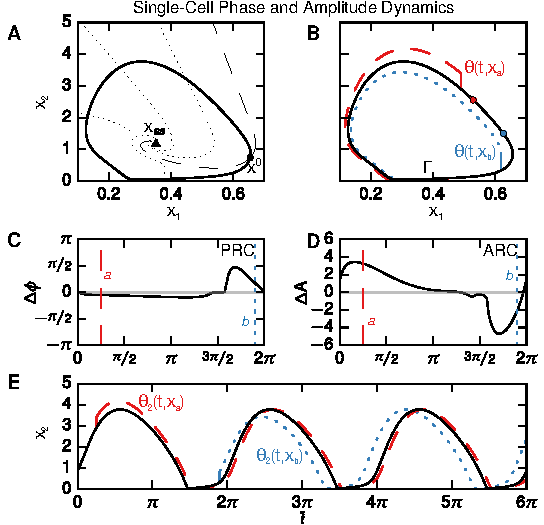
\includegraphics[width=90mm]{chap1/figures/figure_2_prc_arc.pdf}
    \end{center}
    \caption{Phase and amplitude response curves for a single two-state limit cycle oscillator model (from \cite{Novak2008}) describing oscillator response to perturbation.
    (\textbf{A}) Phase breakdown of state space, as visualized through isochrons: sets of points with constant phase within state-space \cite{Doyle2006}.
    The isochron with phase $\phi=0$ is shown as the dashed line, with each subsequent (dotted) isochron at intervals of $\frac{T}{5}$.
    The fixed point ($x_{ss}$) and a reference point on the limit cycle ($x^0$) are shown with a triangle and a circle, respectively.
    (\textbf{B}) State-space response to an identical perturbation $\Delta x$ at phases $\phi = 0.125T$ (trajectory $\theta_a(t,x_a)$, dashes) and $\phi = 0.95T$ (trajectory $\theta_b(t, x_b)$, dots).
    The final phase angle at which each trajectory returns to $\Gamma$ are shown by circles, indicating a phase delay for $\theta_a$ and phase advance for $\theta_b$.
    Perturbation $a$ results in an amplitude increase (i.e. is perturbed to the outside of $\Gamma$), while $b$ results in a decrease.
    (\textbf{C}) Phase and
    (\textbf{D}) amplitude response curves for the perturbation $\Delta x$. 
    (\textbf{E}) Time-domain representation of state $x_2$, demonstrating phase and amplitude responses relative to limit cycle path $\tilde\gamma(\tilde{t},x^0)$ (black solid line).
    \label{fig:lco}}
\end{figure}

\subsection*{Mathematical treatment of limit cycle oscillator populations\label{sec:35}}
A population of oscillators may be treated through a phase-density approach, as is common 
for phase-only models \cite{Ukai2007, StJohn2014b}.
Phase-only oscillator models use a single differential equation for the phase of each oscillator within a population,
and capture population dynamics through coupling terms in these equations.
To maintain consistency with these phase-only approaches, it is important to use the definition of phase $\phi\in[0,2\pi)$.
Furthermore, it is convenient to use the rescaling:
\begin{equation}
    \tilde{t} = \omega t
\end{equation}
\begin{equation}
    \tilde{f} = f/\omega
\end{equation}
\begin{equation}
    \frac{dx}{d\tilde{t}} = \tilde{f}(x(\tilde{t}), p)
\end{equation}
\begin{equation}
    \tilde{\gamma}(\tilde{t}, x_0) = \gamma(t,x_0)
\end{equation}
\begin{equation}
    \tilde{\theta}(\tilde{t}, x_a) = \theta(t,x_a)
\end{equation}
which yields a periodicity of $T=2\pi$ to simplify circular statistics and maintain consistency with \cite{StJohn2014b}.
Importantly, this does not affect our phase mapping.
The total number of oscillators is conserved, so
\begin{equation}
    \int_0^{2\pi} p(\phi,\tilde{t}) d\phi = 1.
\end{equation}
The exact phase probability density function $\hat{p}(\phi,\tilde{t})$ following a perturbation  may be calculated exactly by using a change of variables:
\begin{equation}
    \hat{p}(\phi,\tilde{t})dg(\phi) = p(\phi,\tilde{t})d\phi,
\end{equation}
where $p(\phi,\tilde{t})$ is the phase probability density function prior to perturbation, 
and $g(\phi) = \phi+\Delta\phi$ is the phase transition curve, a mapping of oscillator phase 
before perturbation to phase following perturbation.
However, in the limit of a large oscillator population ($n\to\infty$) it is simpler to map 
the distribution of phases in the population using a complex variable $z$, given by
\begin{equation}
    \begin{split}
    z &=\rho \mathrm{e}^{i\bar{\phi}}\\
      &= \frac{1}{N}\sum_{j=1}^N \mathrm{e}^{i\phi_{j}},
    \end{split}
\end{equation}
where $\bar{\phi}$ is the mean phase and $\rho$ is called the Kuramoto order parameter, 
also called the synchronization index.
The Kuramoto order parameter is related to the population variance and yields a simpler 
calculation at the expense of some detail regarding the exact distribution of phases
(for additional detail, see \cite{kuramoto1984}).
For a perfectly synchronized population, $\rho=1$, and for a population uniformly distributed on $[0,2\pi)$, $\rho=0$.
The population phase and amplitude responses may be then calculated by
\begin{equation}
    \Delta\bar{\phi} = \angle z - \angle\hat{z},
\end{equation}
and
\begin{equation}
    \Delta\rho = |z| - |\hat{z}|,
\end{equation}
respectively, where
\begin{equation}
    z = \int_0^{2\pi} \mathrm{e}^{i\phi}p(\phi,\tilde{t})d\phi,
\end{equation}
\begin{equation}\label{eq:zhat}
    \hat{z} = \int_0^{2\pi} \mathrm{e}^{i\phi}\hat{p}(\phi,\tilde{t})d\phi = \int_0^{2\pi} \mathrm{e}^{ig(\phi)}p(\phi,\tilde{t})d\phi.
\end{equation}


\subsubsection*{Phase diffusion of uncoupled oscillators and population-scale mean expression profiles}
Even for an identical population of oscillators, intrinsic cycle-to-cycle variability in period length will effect a gradual desynchronization over time.
The drift of phases due to stochastic noise is approximately diffusive \cite{Gonze2002, Gonze2006, Teramae2004, StJohn2014b}, and so the evolution of the phase probability density function may be described through a Fokker-Planck equation:
\begin{equation}\label{eq:convdiff}
    \frac{\partial p}{\partial \tilde{t}} = \frac{\partial p}{\partial \phi} +D\frac{\partial^2 p}{\partial\phi^2},
\end{equation}
where $D\frac{\partial^2 p}{\partial\phi^2}$ describes phase diffusion about $[0,2\pi)$ the with diffusion coefficient $D$, and $\frac{\partial p}{\partial\phi}$ describes convection of mean phase around $[0,2\pi)$.
Note that \eqref{eq:convdiff} has periodic boundary conditions and an initial condition $p(\phi,0) = \Psi(\phi)$, yielding the solution as a convolution of the initial conditions with a wrapped normal distribution:
\begin{equation}\label{eq:convdiffsol}
    p(\phi,\tilde{t}) = \Psi(\phi)*f_{WN}(\phi; \tilde{t}, \sqrt{2D\tilde{t}}),
\end{equation}
where $f_{WN}$ is the wrapped normal distribution, $\tilde{t}$ is the mean phase (due to our rescaling), and $\sqrt{2D\tilde{t}}$ is the standard deviation of phase \cite{StJohn2014b}.
This convolution may be simplified by approximating $\Psi(\phi)$ as a normal distribution with mean $\mu_0$ and standard deviation $\sigma_0$, to yield
\begin{equation}
    p(\phi,\tilde{t}) = f_{WN}(\phi; \mu_0+\tilde{t}, \sqrt{\sigma_0^2 + 2D^2\tilde{t}^2}).
\end{equation}

The population-scale mean expression of state $i$, $\bar{x}_i(\tilde{t})$, for oscillators on the limit cycle $\Gamma$ can be found through a weighted average of the phase probability density function:
\begin{equation}\label{eq:diff}
    \bar{x}_i(\tilde{t}) = \int_0^{2\pi} \gamma(\phi,x^0) p(\phi,\tilde{t}) d\phi
\end{equation}
where $x^0$ is the point on $\Gamma$ where $\phi=0$.
It is important to note that our rescaling leads to a linear relationship between $\phi$ and $t$, and thus integration from $\phi=0$ to $2\pi$ is the equivalent of integration from $t=0$ to $T$.
For the case where limit cycle trajectory $\tilde{\gamma}(\tilde{t}, x^0) = \cos(\tilde{t})$, and where the phase probability density function evolves according to the convection-diffusion equation \eqref{eq:convdiff},  then \eqref{eq:diff} yields an exponentially-damped sinusoidal result \cite{StJohn2014b}:
\begin{equation}
    \bar{x}_i(t) = \mathrm{e}^{-D\tilde{t}}\cos(\, \tilde{t} \,),
\end{equation}
consistent with both experimental and computational studies \cite{Welsh2004, Rougemont2007, StJohn2015}.
Non-sinusoidal limit cycles will also approach this trajectory, as phase diffusion will damp higher frequency sinusoidal components of the limit cycle \cite{StJohn2014b}.

The population-scale mean expression after a perturbation may be calculated by decomposing the perturbed trajectory $\hat{x}_i(\tilde{t})$ into the steady-state perturbed trajectory  $\hat{x}_{i,SS}$ resulting from the condensing or dispersing of phases along the limit cycle, and the transient population-scale deviations from the limit cycle $\hat{x}_{i,trans}$ which eventually converge to $0$. 
The steady-state trajectory is 
\begin{equation}
    \hat{x}_{i,SS}(\tilde{t}) = \int_{0}^{2\pi} \tilde{\gamma}_i(\phi, x^0)\hat{p}(\phi,\tilde{t})d\phi,
\end{equation}
where $\hat{p}(\phi,\tilde{t})$ must be calculated numerically for short times immediately following the perturbation, but may be approximated by \eqref{eq:zhat} for sufficient damping.
The transient trajectory necessitates the definition of the deviation trajectory:
\begin{equation}
    \delta x_i(\phi,\tilde{t}) = \tilde{\theta}_i(\tilde{t})-\tilde{\gamma}_i(\tilde{t}+\phi+\Delta\phi, x^0),
\end{equation}
which represents the distance between the perturbed trajectory and the limit cycle trajectory to which it converges.
The average transient affect can then be calculated by weighting the deviation term by the phase probability density prior to perturbation:
\begin{equation}
    \hat{x}_{i,trans}(\tilde{t}) = \int_0^{2\pi} \delta x_i(\phi,\tilde{t})p(\phi,\tilde{t})d\phi.
\end{equation}
Finally, the population-scale mean expression profile, $\hat{x}_i(\tilde{t})$, is
\begin{equation}
    \hat{x}_i(\tilde{t}) = \int_{0}^{2\pi} \left( \tilde\gamma_i(\phi, x^0)\hat{p}(\phi,\tilde{t}) + \delta x_i(\phi,\tilde{t})p(\phi,\tilde{t}) \right)d\phi,
\end{equation}
as in \cite{StJohn2014b}.
Example population phase and amplitude response dynamics are shown in Figure \ref{fig:pop}.

\begin{figure}[p] 
    \begin{center}
        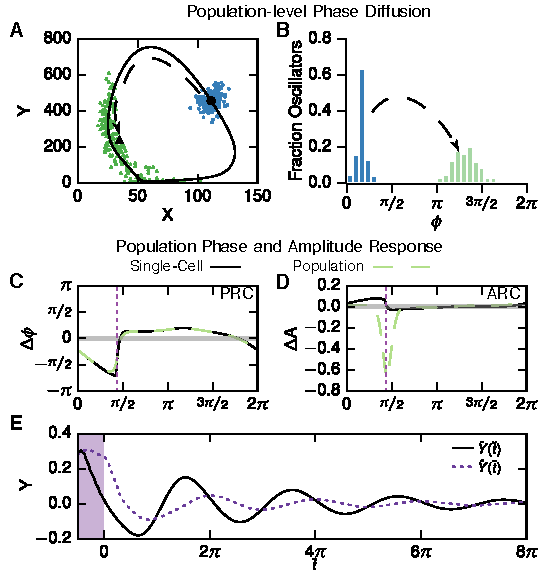
\includegraphics[width=90mm]{chap1/figures/figure_3_population.pdf}
    \end{center}
    \caption{Phase and amplitude response dynamics for a population of two-state limit cycle oscillator models from \cite{Novak2008}.
    (\textbf{A}) State-space representation of phase diffusion. An initial population of 200 oscillators (circles, blue) was simulated stochastically for $\frac{T}{2}$ resulting in a dispersion of final phases (triangles, green). The average molecular count of $X$ and $Y$ for initial and final conditions are shown in bold. The movement of the center of mass toward the inside of limit cycle orbit $\gamma$ reflects amplitude damping due to desynchronization.
    (\textbf{B}) The diffusion of phases due to intrinsic noise is shown as a histogram of phases for the simulation from panel A.
    (\textbf{C} and \textbf{D}) Single-cell (solid line) and population (dashed line) PRC and ARC, for a temporary $40\%$ increase in parameter $k_2$. 
    (\textbf{E}) Population-scale mean expression profile $\hat{Y}(\tilde{t})$ resulting from perturbation at the phase indicated in panels B and C (dotted line in both panels).
    This results in a phase lag, and a loss of amplitude in comparison to the unperturbed trajectory $\bar{Y}(\tilde{t})$ due to the desynchronizing effect of the pulse, despite negligible changes in single-cell amplitude. 
\label{fig:pop}}
\end{figure}


\section{Taking control of the clock}

\begin{figure}[p]
    \begin{center}
        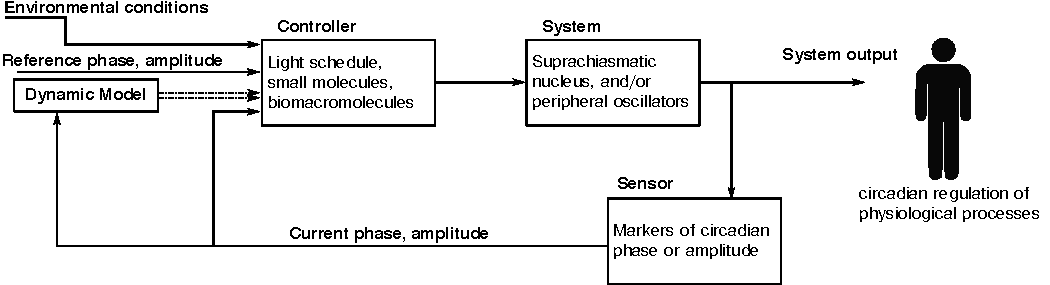
\includegraphics[width=180mm]{chap1/figures/figure_4_simple_control_scheme.pdf}
    \end{center}
    \caption{A generalized scheme for feedback control of the circadian clock identifying essential components and possible control variables. This diagram is generalizable to a variety of desirable control outcomes (optimal entrainment, phase shifting, amplitude) and control vectors (light, pharmaceuticals). A feed-forward scheme could be similarly implemented by shifting the clock in anticipation of a disturbance, such as light exposure during night.    \label{fig:control}}
\end{figure}

    Control of biological systems may be studied as either ``open-loop'' optimal control in which system model behavior is optimized, or ``closed-loop'' feedback control in which feedback from sensing the process itself updates the actuation of the process.
A coalescing of control engineering and systems biology has resulted in widespread use of open-loop and feedback control approaches in various biological and biomedical applications~\cite{Lauffenburger2000, Bailey2005}.
These include identifying and modulating cellular behavior~\cite{Julius2008, Perley2014, Yan2017}, treating diseases~\cite{ElSamad2005, Gondhalekar2016}, constructing synthetic biological circuits~\cite{Chen2013, DelVecchio2017}, optimizing biomanufacturing productivity \cite{Craven2014, Giordano2016}, and formulating targeted drug delivery systems~\cite{Haddad2003, Luni2011, Yu2017, Jin2017}.
Unlike open-loop systems that require manual intervention at critical times to prevent deleterious outcomes, closed-loop drug delivery systems enable effective regulation of targeted biological pathways by leveraging control-relevant models, systematic prediction, or decision-making based on clinical targets.
Therefore, these approaches have found use in manufacturing and medical devices.
Additional improvements in the quality of closed-loop drug delivery and adherence within society has been fueled by the invention of wearable sensors~\cite{Amendola2014}, minimally invasive actuators, and embedded decision-making platforms~\cite{Zavitsanou2016}, along with novel drug delivery mechanisms~\cite{Qiu2017} or input-output pairs~\cite{Bakh2017}.

    Leveraging computational models of the circadian clock and the mathematical tools outlined previously, it is possible to formulate control approaches for the manipulation of clock phase, clock amplitude, or entrainment.
    For example, open-loop control has been applied to light resetting of the human clock \textit{in silico} \cite{Serkh2014, Zhang2016}.
    Feedback control has also been implemented \textit{in silico}, for example, on the drosophila clock \cite{Bagheri2007, Bagheri2008a}, or as proportional or proportional-integral feedback control laws derived from optimal control \cite{Efimov2009}.
    Figure~\ref{fig:control} shows the overarching scheme by which the clock may be controlled either \textit{in vivo}, \textit{in vitro}, or \textit{in silico}.
In general, such a control system consists of a sensor tasked with observing the system state, an actuator by which control is exerted, and a control algorithm connecting these parts.
Here, we briefly introduce the sensor and actuator components of a feedback control strategy.
In Section II, I provide a more thorough review of the literature regarding design of circadian control algorithms and present two original studies of controller design for manipulating circadian phase and synchrony.



\subsection*{Sensor design}
A critical component of a circadian control system is the design of a sensor which can accurately assess circadian phase while remaining minimally invasive.
Current markers of human circadian phase are plasma or saliva melatonin, plasma cortisol, or core body temperature \cite{Klerman2002}.
More recent works have utilized ambulatory monitoring approaches, using variables such as motion, respiration, light exposure, and ECG, and fitting a multivariate model, with some success \cite{Kolodyazhniy2011}.
However, these current approaches are likely too invasive for everyday use.
Furthermore, single-dimensional recordings such as melatonin provide limited resolution for tracking phase, such as during daytime when melatonin concentration is negligible.
Enabled by smartphone technology, another possible route to sensing circadian phase would be actigraphy in conjunction with a calculated light schedule \cite{Walch2016}.
However, these metrics would necessitate a robust control algorithm to compensate for potential sensor error.
In general, the performance of any control algorithm would be highly subject to sensor accuracy, and choice of a sensor remains an open research question.

\subsection*{Actuator design}
\subsubsection*{Photic actuation}
The most common route to artificial control of the clock is through the natural control variable: light.
This path is favorable as it is non-invasive and the mechanistic pathway is relatively well-understood.
Historically, many studies have examined the role of light in entraining the clock.
Recent studies have also begun to examine closing the loop between sensing and control of the clock by calculating an optimal light profile for reentrainment \cite{Serkh2014, Walch2016}.
Potential downsides to using light in clock control include delays in responsiveness, as the system is not evolutionarily optimized to respond to large shifts in phase rapidly; and loss of control during ``dead zones,'' where light has little effect on circadian phase \cite{Dunlap2004}.


\subsubsection*{Pharmacological actuation}
Small-molecule modulators of the circadian clock have gained significant recent attention \cite{Hirota2010, Hirota2012a, StJohn2014a}.
Small-molecule pharmaceuticals are attractive due to facile delivery and uptake and ability to target specific proteins or complexes within the clock.
Two such molecules, KL001 and Longdaysin, have been identified via high-throughput screening methods.
Identifying the mechanistic action of these clock modulators presents a unique challenge, due to the inherent complexity of the gene regulatory network obscuring the direct effect.
Neurotransmitters, or pharmaceuticals which modulate neurotransmitter expression, offer another possible path to control of the circadian oscillator.
In particular, the neurotransmitters VIP and GABA have attracted attention, due to their preeminent role in synchronizing the SCN \cite{An2013,Kingsbury2016}.
However, these neurotransmitters are also implicated in a variety of non-circadian functions, and may not be sufficiently precise to target solely the clock.
An important limitation on the potential of molecular clock modulators is that the oscillator appears to be optimized for high-amplitude high-precision rhythms, and very few clock modulations are able to simultaneously increase amplitude and precision for an extended duration \cite{StJohn2015}.
This suggests that any long-term (i.e.~many-cycle) clock modulation might be best accomplished by a dynamic approach, where circadian amplitudes are increased by precisely timing the administration of a clock-modulating therapeutic.



\section{Conclusions}
The mammalian circadian system is a natural, multi-scale, robust control system with widespread influence over metabolism and behavior.
In the past two decades, a systems engineering approach has yielded great insight into the mechanistic function of the mammalian circadian oscillator.
As technology for sensing and actuating circadian function continues to develop, control theory also will play an important role in developing novel clock therapies.
Furthermore, design principles for generating stable control from sloppy biological components may yield improvements in the design of artificial control strategies, or in the design of artificial genetic circuits in synthetic biology.












% NOTES:
% text and figure notation : fix it
